\documentclass[11pt]{article}
\usepackage[utf8]{inputenc}
\usepackage[english]{babel}
%\usepackage{fancyhdr}
%\usepackage{dsfont} %eins als neutrales element
%\renewcommand{\rmdefault}{ppl}
%\usepackage{caption,chngcntr}
%!TeX spellcheck = en_US 
\usepackage{libertine}

\usepackage{hyperref}
\usepackage{mathrsfs}
\usepackage{enumitem} 
\usepackage{paralist}
\usepackage[ 
left=2.5cm,    
right=2.5cm,
top=2cm,
bottom=2cm,
]{geometry}

\usepackage[labelfont={},font={footnotesize}]{caption}

\renewcommand{\figurename}{Fig.}
\renewcommand{\tablename}{Tab.}

%\numberwithin{table}{section}
%\numberwithin{figure}{section}
%\numberwithin{equation}{section}

\usepackage{array}
\newcolumntype{L}[1]{>{\raggedright\let\newline\\\arraybackslash\hspace{0pt}}m{#1}}
\newcolumntype{C}[1]{>{\centering\let\newline\\\arraybackslash\hspace{0pt}}m{#1}}
\newcolumntype{R}[1]{>{\raggedleft\let\newline\\\arraybackslash\hspace{0pt}}m{#1}}

\usepackage{fancybox} 
\usepackage[T1]{fontenc} 

\usepackage[arrow, matrix, curve]{xy}
\usepackage{amsthm}
\usepackage{paralist}
%\usepackage{graphicx} 
%\usepackage{tabularx}
\usepackage{amssymb}
\usepackage{amsmath}


\usepackage{setspace}	
\setstretch{1.2}
\usepackage{natbib}
\bibliographystyle{apalike}

%tikz
\usepackage{tikz}
\usetikzlibrary{shapes.geometric, arrows}
\usetikzlibrary{arrows, arrows.meta, calc, positioning, quotes, shapes}
\usetikzlibrary{automata,positioning}
\usetikzlibrary{positioning, arrows}
\usetikzlibrary{decorations.pathmorphing}
\usetikzlibrary{calc}
\usetikzlibrary{matrix}


\usepackage{float}
\setlength{\parindent}{0pt} 

\definecolor{madrid}{rgb}{0.2,0.2,0.8}
\definecolor{darkgreen}{rgb}{0.2,0.6,0.2}
\definecolor{darkred}{rgb}{0.8,0.2,0.4}
\definecolor{orange}{rgb}{0.9,0.4,0.0}

%\theoremstyle{definition}
%\newtheorem{theorem}{Theorem}
%\newtheorem{definition}{Definition}
%\usepackage{varioref}


\begin{document}
	
 

	
	
	\section{Multiresolution decomposition}
	features of MRD that are not inherent in the Fourier decomposition according to \citet{Howell1997}:
	\begin{compactenum}
		\item[-] the peak in multiresolution cospectra depends
		mostly on the width of the dominant (local) flux events whereas the wavelength
		of the peak in Fourier cospectra depends on the principal periodicity
		\item[-] Each mode of the multiresolution decomposition corresponds to a simple unweighted (nonoverlapping) moving average and thus, satisfies the rules of
		Reynolds averaging.
		\item[-] N arithmetic operations (compared to N log(N) for FFT)
		\item[-] Each mode of the multiresolution decomposition corresponds to a simple unweighted (nonoverlapping) moving average and thus, satisfies the rules of
		Reynolds averaging.
	\end{compactenum}
	
	
	
	\begin{figure}[H]
		\small
		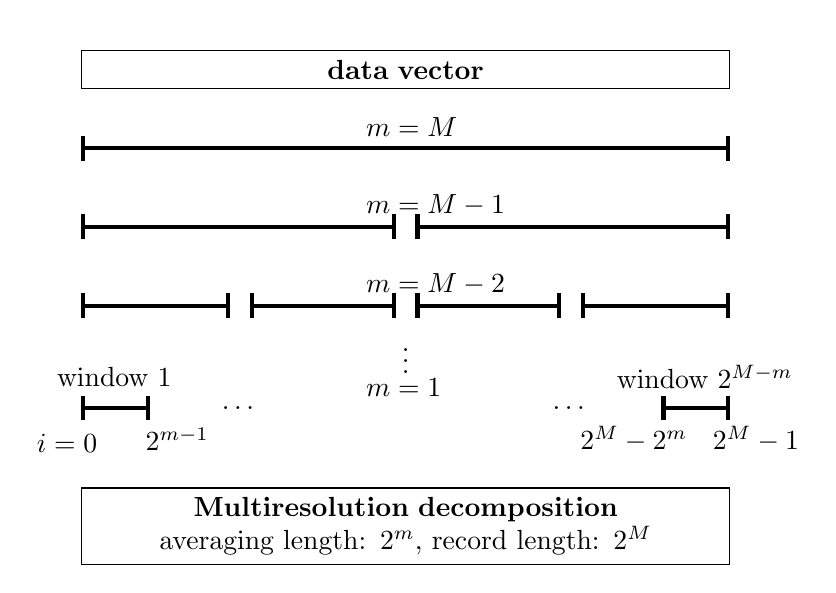
\begin{tikzpicture}
			\node(start)  [draw, text width = 8cm,align=center] at (0,0)  {\textbf{data vector}};
			\node(mrd)  [draw, text width = 8cm,align=center] at (0,-5.8)  {\textbf{Multiresolution decomposition} \\
			averaging length: $2^{m}$, record length: $2^{M}$};
			\node(h1) at (-4.25,0)  {};
			\node(h2) at (4.25,0)  {};
			\node(h3) at (0,0)  {};
			\node(h4) at (-2.1,0)  {};
			\node(h5) at (2.1,0)  {};
			\node(h6) at (-3.125,0)  {};
			\node(h7) at (3.125,0)  {};
			\node(dots) at (0,-3.6)  {$\vdots$};
			\node(dots2) at (-2.1,-4.3)  {$\dots$};
			\node(dots3) at (2.1,-4.3)  {$\dots$};
			\draw[|-|,line width=1.5pt,text width=5cm, align=left,transform canvas={yshift=-10mm}] (h1) -- (h2) node [above] at (2,0) {$m=M$} ;
			\draw[|-|,line width=1.5pt,text width=5cm, align=left,transform canvas={yshift=-20mm}] (h1) -- (h3) node [above] at (2,0) {$m=M-1$} ;
			\draw[|-|,line width=1.5pt,text width=5cm, align=left,transform canvas={yshift=-20mm}] (h2) -- (h3);
			
			\draw[|-|,line width=1.5pt,text width=5cm, align=left,transform canvas={yshift=-30mm}] (h1) -- (h4)
			node [above] at (2,0) {$m=M-2$};
			\draw[|-|,line width=1.5pt,text width=5cm, align=left,transform canvas={yshift=-30mm}] (h3) -- (h4);
			\draw[|-|,line width=1.5pt,text width=5cm, align=left,transform canvas={yshift=-30mm}] (h3) -- (h5);
			\draw[|-|,line width=1.5pt,text width=5cm, align=left,transform canvas={yshift=-30mm}] (h2) -- (h5);
			
			\draw[|-|,line width=1.5pt,text width=5cm, align=left,transform canvas={yshift=-43mm}] (h1) -- (h6)
			node [above] at (2,0) {$m=1$};
			\draw[|-|,line width=1.5pt,text width=5cm, align=left,transform canvas={yshift=-43mm}] (h2) -- (h7);
			
			
			\node(i0) at (-4.3,-4.75)  {$i=0$};
			\node(i1) at (-2.9,-4.7)  {$2^{m-1}$};
			\node(i2) at (2.9,-4.7)  {$2^{M}-2^{m}$};
			\node(im) at (4.45,-4.7)  {$2^{M}-1$};
			\node(w1) at (-3.7,-3.9)  {window 1};
			\node(wm) at (3.8,-3.9)  {window $2^{M-m}$};
		\end{tikzpicture}
		\centering
		\caption{Schematic visualization of the multiresolution decomposition procedure according to \citet{Howell1997}.}
	\end{figure}
	
	
	

\end{document}